% THIS IS SIGPROC-SP.TEX - VERSION 3.1
% WORKS WITH V3.2SP OF ACM_PROC_ARTICLE-SP.CLS
% APRIL 2009
%
% It is an example file showing how to use the 'acm_proc_article-sp.cls' V3.2SP
% LaTeX2e document class file for Conference Proceedings submissions.
% ----------------------------------------------------------------------------------------------------------------
% This .tex file (and associated .cls V3.2SP) *DOES NOT* produce:
%       1) The Permission Statement
%       2) The Conference (location) Info information
%       3) The Copyright Line with ACM data
%       4) Page numbering
% ---------------------------------------------------------------------------------------------------------------
% It is an example which *does* use the .bib file (from which the .bbl file
% is produced).
% REMEMBER HOWEVER: After having produced the .bbl file,
% and prior to final submission,
% you need to 'insert'  your .bbl file into your source .tex file so as to provide
% ONE 'self-contained' source file.
%
% Questions regarding SIGS should be sent to
% Adrienne Griscti ---> griscti@acm.org
%
% Questions/suggestions regarding the guidelines, .tex and .cls files, etc. to
% Gerald Murray ---> murray@hq.acm.org
%
% For tracking purposes - this is V3.1SP - APRIL 2009

\documentclass{sig-alternate}
\usepackage{amstext}
\usepackage{pdfpages}
\usepackage{alltt}
\usepackage{epstopdf}
\usepackage{xspace,colortbl}
\usepackage[USenglish]{babel}
\usepackage{multirow}
\usepackage{url}
\usepackage{subfigure}
\usepackage{graphicx}
\usepackage{amssymb}
\usepackage{fmtcount}
\usepackage{amsfonts}
\usepackage{xspace}
\usepackage{amsmath}
\usepackage{multirow}
\usepackage[mathscr]{eucal}
%\usepackage{psfrag}
\usepackage{colortbl}
\usepackage{bm}
\usepackage[nospace]{cite}
\makeatletter
\newif\if@restonecol
\makeatother
\let\algorithm\relax
\let\endalgorithm\relax
\usepackage[lined,boxed,vlined,ruled]{algorithm2e}
\usepackage[skip=1pt,font=bf]{caption}
\special{papersize=8.5in,11in}

\makeatletter
\def\@copyrightspace{\relax}
\makeatother

\begin{document}

\title{Social Influence Bias in Recomender Systems: A Non-Parametric Analysis of Multi-valued Data From the California Report Card}

\linespread{0.95}%
\setlength{\belowdisplayskip}{2pt} \setlength{\belowdisplayshortskip}{2pt}
\setlength{\abovedisplayskip}{2pt} \setlength{\abovedisplayshortskip}{2pt}
\selectfont

%
% You need the command \numberofauthors to handle the 'placement
% and alignment' of the authors beneath the title.
%
% For aesthetic reasons, we recommend 'three authors at a time'
% i.e. three 'name/affiliation blocks' be placed beneath the title.
%
% NOTE: You are NOT restricted in how many 'rows' of
% "name/affiliations" may appear. We just ask that you restrict
% the number of 'columns' to three.
%
% Because of the available 'opening page real-estate'
% we ask you to refrain from putting more than six authors
% (two rows with three columns) beneath the article title.
% More than six makes the first-page appear very cluttered indeed.
%
% Use the \alignauthor commands to handle the names
% and affiliations for an 'aesthetic maximum' of six authors.
% Add names, affiliations, addresses for
% the seventh etc. author(s) as the argument for the
% \additionalauthors command.
% These 'additional authors' will be output/set for you
% without further effort on your part as the last section in
% the body of your article BEFORE References or any Appendices.

\numberofauthors{3} %  in this sample file, there are a *total*
% of EIGHT authors. SIX appear on the 'first-page' (for formatting
% reasons) and the remaining two appear in the \additionalauthors section.
%\author{Sanjay Krishnan,Jay Patel,Ken Goldberg}

%

% Just remember to make sure that the TOTAL number of authors
% is the number that will appear on the first page PLUS the
% number that will appear in the \additionalauthors section.

\maketitle
\begin{abstract}
Almost all recommender systems display aggregate statistics before participants enter ratings.
These statistics can bias a participant's decision and is known as Social Influence Bias.
We explore this bias in a new platform, the California Report Card (CRC), which reveals the median values to participants after they assign ratings, and allows them to modify their ratings.
We hypothesized that this will lead to revised ratings closer to the revealed median.
We develop a non-parametric significance testing framework based on the Wilcoxon rank-sum statistic to test this hypothesis, and compare our results to a randomized SurveyMonkey survey asking the same questions as the CRC. 
We learn a predictive model relating a participant's initial rating, the observed median, and the rating change, using a polynomial regression technique and Bayesian Information Criterion optimal model search.
Our results suggest statistically significant movement towards the median value for the particpants who changed their ratings.
We learned the optimal polynomial model on ratings for six questions, four of which were modeled with linear functions.
The two remaining questions, about the implementation of Obamacare and Same-sex Marriage Rights in California, were modeled as quadratic functions with significantly higher downward tendency for ratings higher than the median.
We applied the predictive model to infer initial ratings from finals ones and showed that could ``correct" the rating distribution by 76.3\%.
The CRC, our data, and experimental code can be found at:
http://californiareportcard.org
https://github.com/BerkeleyAutomation/socialInfluence
\end{abstract}

% A category with the (minimum) three required fields
%\category{H.4}{Information Systems Applications}{Miscellaneous}
%A category including the fourth, optional field follows...
%\category{D.2.8}{Software Engineering}{Metrics}[complexity measures, performance measures]

%\terms{Theory}

%\keywords{ACM proceedings, \LaTeX, text tagging} % NOT required for Proceedings

\section{Introduction}

In the 1950's, Solomon Asch performed a well-known series of experiments 
\cite{asch1956studies, asch1955opinions, bond1996culture} where
subjects were asked to choose which of a set of lines matched the
length of a reference line.  
When working in private, only 1\% of choices were incorrect.  
But when answering in the presence of a group of confederates who agreed on incorrect answers, 25\% of participants
conformed to the incorrect consensus.  
These results were widely repeated to confirm what is now known as \emph{social influence bias}:
the tedency for participants to conform with the perceived community ``norm" \cite{demarzo2003persuasion,
moscovici1972social, wood2000attitude}.

In almost all recommender systems, participants see the community ``norm" in the form of 
aggregate statistics (the average or median rating values) before leaving a rating of their own;
potentially introducing social influence bias into the rating data.
This interface paradigm is, of course, reasonable to facilitate browsing and selection in a large lists of items.
For example, online retailers such as Amazon display the average rating value
for products and Netflix displays the average rating value of movies
(Figure \ref{grading-0}).  Display of average ratings values can also be
used as an incentive\cite{jian2012incentive} to reveal information about
peers after a participant enters his or her own grade.  
Display of statistics also increases the perceived transparency of open democracy platforms that encourage political engagement
\cite{albors2008new,o2012transparency,noveck2008wiki}.

\begin{figure}[t]
  \centering
    \includegraphics[scale=0.36]{../plots/intro2.png}
      \caption{Typical displays of aggregate statistics (the average/mean or median rating value) in Amazon, Netflix, and the California Report Card
that can lead to social influence bias.}
      \label{grading-0}
\end{figure}

Susceptibility to influence has been studied in the context recommender systems \cite{cosley2003seeing}, and, in particular, Cosley et al. explored
different rating scenarios and how system-generated rating predictions may influence participant ratings.
They found that in a variety of scenarios including presenting manipulated predictions, presenting predictions on already rated items, and changing the rating scale had statistically significant influence on participants ratings.
These results motivate a study of social influence bias in recommender systems which, in contrast, can arise organically from the community rather than
from a prompt from the system, such as a prediction.
Conformity can yield ratings that are closer to the average, less diverse, and less representative of participants' true
evaluations for items, which can in turn affect similarity measures between items and users.  

In this paper, we propose a methodology to learn, analyze, 
and mitigate the effects of social influence bias in recommender systems.  
As a case study, we evaluate our methodology on a new recommender system, the 
California Report Card (CRC).
In the CRC, participants assign ratings (letter grades A+ to F, a 13 point
scale) to the State of California on six political issues.  
Then, the CRC uses the ratings to place participants in a open-ended
political discussion with an initial set of comments from those who 
rated the state most similarly.
Conformity ratings of the state can degrade the performance of the ``recommendation", 
a set of comments from like-minded participants.

However, the CRC has novel interface that allows us to learn the effects of Social Influence Bias.
The CRC interface reveals median grade values to participants \emph{after} they enter
their own rating and then allows participants to revise their
rating.
The key insight is that the combination of initial and revised ratings
pairs allows us to determine if the social influence bias is
statistically significant, and if so, can be used to build an
inference model that can predict the biasing tendency; thus mitigate the bias 
in a dataset of already biased ratings.  

Our methodology has three main components:
\vspace{1em}

\noindent \textbf{Learn} To initialize with baseline data, an initial
``learning" phase asks an initial set of participants to rate a set of
items twice: before seeing the median rating, and again after the
median is revealed.  This collects triplets of ratings for each
participant (initial rating, median rating, and final rating).

\vspace{1em}

\noindent \textbf{Analyze} Given these triplets, we propose a new
nonparametric significance test based on the Wilcoxon statistic to
determine whether ratings that were changed are significantly closer
to the median, i.e. the degree of social influence bias for each item.

\vspace{1em}

\noindent \textbf{Mitigate} Using the Bayesian Information Criterion
(BIC), we learn a polynomial function of optimal degree that estimates
the initial rating from the final rating and the median. This can be
used in a post-learning phase (when medians are always visible), or on
historical ratings, to estimate what a participant's rating would be
without social influence bias.

\vspace{1em}

A key priority is a nonparametric approach to modeling 
social influence bias. Many earlier studies of social influence
bias have focused on binary ratings (eg. up or down) \cite{muchnik2013social, zhu2012switch}.  
However, recommender systems often have multi-valued rating scales (eg. 5 stars), 
and parametric significance tests (eg. t-test and $\chi^2$ test), as used in
\cite{cosley2003seeing}, often have poor performance in this setting.
We further show how model-search methods such as BIC can be used to model
possible Social Influence Bias without having to make a strong assumption 
about structure of the bias (eg. linear, conforming vs. contrarian).

%estimate
%unbiased ratings and present results with data from the California
%Report Card, including learning curves that show that in most cases
%estimation converges relatively quickly.  Applying the proposed
%methodology to existing recommender systems raises a number of interesting
%questions for further research.

%In our case study, we apply this methodology to the California Report
%Card (CRC), a two-part recommender system that encourages political
%engagement.  In Part I, participants assign letter grades (a 13-point
%rating scale) to the state of California on six political issues.
%Part I uses the six ratings to quantify similarity between
%participants and issues.  In Part II, participants enter textual
%suggestions about new political issues and grade the suggestions of
%other participants.  Part II uses participant ratings to identify
%(recommend) valuable suggestions.  The CRC was announced via press and
%social media in late January 2014.

Results to date from the CRC suggest that given the opportunity, many
participants will revise their grades/ratings: $862$ out of $9390$
ratings were changed after participants saw the median value.  We
found statistically significant effects of social influence bias, with
ratings on average 19.3\% closer to the median value than ratings that
were not changed.  We also conducted an independent reference survey
using SurveyMonkey to ask a random sample of 611 participants from the
company's paid pool of California participants to grade the same set
of issues without displaying the median values.  This data did not
exhibit the same clustering around the median as the CRC, which
comparably had ratings that were statistically significantly closer to
the median (12.0\%), suggesting that social influence bias is an
important factor.

%We study social influence bias in this platform, especially since tendency to conform will affect our measure of similarity between participants in phase one.

%To minimize assumptions about the statistical distribution of ratings, we develop a non-parametric approach to test the following social influence hypotheses:

%\noindent \textbf{- Hypothesis 0} Given the opportunity, participants will revise their ratings.

%\noindent \textbf{- Hypothesis 1} When a participant does change a rating it will be in the direction that conforms to the presented median.

%\noindent \textbf{- Hypothesis 2} Participants will become more moderate in their ratings if they observe that their ratings consistently are in disagreement with the population consensus.

%Nearly 35\% of participants changed at least one rating, and our study finds statistically significant effects of social influence bias in the $862$ out of $9390$ ratings which were changed after participant's saw the median value.
%To further model patterns of participant behavior, we train a polynomial regression with the Bayesian Information Criterion (BIC) that predicts rating changes given a participant's current rating.
%The model can also be inverted to infer initial ratings from final ones.
%Prior results in social influence bias have focused on binary rating systems eg. up or down votes \cite{muchnik2013social, zhu2012switch}.
%However, these models are not directly applicable in many recommender systems which often have discrete mutli-valued rating scales (eg. 5 stars).

%Our results, which especially focus on mutli-valued ratings, have the following implications for interface and algorithmic design in recommender systems.
%Few existing tools collect both an initial (with the mean/median hidden) and a final rating.
%As seen in the CRC, given the opportunity to revise ratings, many participants will, and it can be informative to collect the pairs of ratings.
%The pairs can reveal more information about participants' initial perceptions, allow us to classify participants as likely to conform/deviate, and also assess the magnitude of social influence from the community.

%Existing recommender systems, can use our models to mitigate these effects, by training on set of rating pairs collected after-the-fact, and then applying the model to infer past participant's ``unbiased" ratings.


\section{Related Work}

%% In the context of recommender systems, social influence has been studied primarily in order to use information about social and trusted friend networks to improve recommendations. Jamali et al. described a stochastic block model which predicts recommendations based on both social relations and rating behavior [A]. Shang et al. described models for for improving recommendations among individuals using the theory of social contagion, and among groups using network theory [B]. Ye et al. proposed a quantification metric of social influence, and proposed probabilstic model to model the decision of item selection [C].

%% However, the Asch model for confirmity suggest a particular biasing effect from an aggregate or ``crowd'' (i.e. the previous raters are anonymous to the current rater). This phenomenon known as social herding ...

The Asch model for conformity is the theoretical basis for \emph{social herding}, the tendency to conform \cite{banerjee1992simple,bikhchandani2000herd}, and herding has been a popular consumer choice model in economics \cite{burnkrant1975informational,dholakia2002auction,huang2006herding}. 
Such models have also been studied in psychology as ``persuasion bias" \cite{demarzo2003persuasion}.
In 2011, Lorenz et al. described how these biases can undermine the effectiveness of crowd intelligence in estimation tasks \cite{lorenz2011social}. 
They argue that social herding causes a diminished diversity of opinion potentially leading to inefficiencies and inaccurate collective estimates.
Danescu-Niculescu-Mizil et al. analyze helpfulness ratings on Amazon product reviews \cite{danescu2009opinions}.
They found that the helpfulness ratings did not just depend on the content of the review but also its aggregate score and its relationship to other scores.
In order to better distinguish social influence from other biases, Muchnik et. al designed a randomized experiment in which comments in an online forum were randomly up-treated or down-treated \cite{muchnik2013social}.
They concluded a statistically significant bias where a positive treatment increased the likelihood of positive ratings by 32\%. 
In both Danescu-Niculescu-Mizil et al. and Muchnik et al., they looked at the problem of Social Influence bias in an a priori setting, where users see the aggregate statistic before giving their rating.
Our work tests for a particular form of social influence where users are given the opportunity to change their opinions following the feedback. 

Zhu et al. conducted an experiment in which users evaluate an image on a subjective question with binary scale (eg. ``Is this image cute?"), which was followed (either immediately or later) by a presentation of the crowd consensus opinion \cite{zhu2012switch}. 
Users were given an opportunity to change their response, and they concluded that there was a significant tendency to change submissions.
The tendency to change was the strongest when users were asked to make their second decision much later and not immediately after the first.
However, Zhu et al. also acknowledge there are competing psychological factors at work in this experiment.
Along these lines, Sipos et al. argue that context along with an aggregate rating plays a large role in the users' ratings. That is, users may attempt to ``correct" the average, by voting in a more polarizing manner (more positively or negatively) \cite{siposreview}.
We extend this prior work to measure and predict these changes when the input is more complex than a binary scale, and propose a non-parametric methodology that can be, in principle, extended to a variety of different input mechanisms.
Our model can also account for a changing aggregate statistic such as a median rating changing as more data is collected. 


%% [A] M. Jamali, T. Huang, and M. Ester, ``A Generalized Stochastic Block Model for Recommendation in Social Rating Networks'', in ACM Conference in Recommender Systems (RecSys'11) , Chicago, IL, USA, October 2011.

%% [B] Shang, Shang, et al. ``Wisdom of the crowd: Incorporating social influence in recommendation models.'' Parallel and Distributed Systems (ICPADS), 2011 IEEE 17th International Conference on. IEEE, 2011.

%% [C] Ye, Mao, Xingjie Liu, and Wang-Chien Lee. ``Exploring social influence for recommendation: a generative model approach.'' Proceedings of the 35th international ACM SIGIR conference on Research and development in information retrieval. ACM, 2012.




\section{The California Report Card}
\subsection{System Description}
The California Report Card (CRC) is a web application that allows participants to advise the state government on timely policy issues.
When participants arrive at the application, they ``grade" the state on following six issues: (1) Implementation of the Affordable Care Act ("Obamacare"),
(2) Quality of K-12 public education, (3) Affordability of state colleges and universities, (4) Access to state services for undocumented immigrants, (5) Laws and regulations regarding recreational marijuana, and (6) Marriage rights for same-sex partners.
Grades are assigned on a thirteen point scale (A+,A,A-,...,D-,F).
These issues are posed in a fixed sequential order each with the same input scale.
Particpants submit grades using a click-and-drag slider interface as illustrated in Figure \ref{grading-1}.
On mobile devices this slider requires the participants to touch and drag their finger to the desired grade.

\begin{figure}[h]
  \centering
    \includegraphics[width=\columnwidth]{../plots/grading-desc-1.png}
      \caption{Grading in the California Report Card. Participants enter grades on six timely issues facing the State of California. After entering their grades, the median grade over all participants is revealed. Participants have the option to change their grades after seeing the median.}
      \label{grading-1}
\end{figure}

Upon release of the slider, the CRC reveals the median grade for that issue over all prior participants.
Even after the median grade is revealed the slider is still active and participants can change their grades.
However, it is important to note that participants were not explicitly told that they could change their grades.
Another important observation is that participants who accessed the application at different times may have seen different median grades as they were calculated based on the data upto that point.
We recorded the initial grade, the median that the participant observed, and any subsequent changes along with timestamps for each of the events. 
Grading all of the six issues was not manditory and participant had the option to skip any of the issues.

The CRC has an additional open-ended discussion phase where participant submit textual suggestions on future issues to include in the report card.
In this work, we focus on the first phase and defer an analysis of biases in the discussion phase to future work.

\subsection{Notation}
To analyze this data, we mapped these 13 grades onto a scale from 0 to 1, with 1 being an A+ and 0 being an F.
Let $P$ denote the set of all participants.
For each participant $p_j\in P$, we associate a 3-tuple of grades ($g_i[j]$, $m[j]$, $g_f[j]$) which represent the initial grade, median observed by the participant, and the final grade.
For each issue, we divided the participants into three subsets of $P$: ones who did not change their grades $P_n$, ones who changed $P_c$, and ones who skipped the question $P_s$.
Our primary objective is to test the distributional properties of rating tuples from participants in $P_n$ compared to those in $P_c$.

To ensure that all participants in the set $P_c$ had an opportunity to see the median grade and then react, we filtered this group using the timestamps. 
The median grade appears in the interface with an animation whose completion time varied between devices, so we set a grace period of 3 seconds before 
we categorized the participant into set $P_c$.  

For consistency, we use the same notation to describe participants in the reference survey. We denote the set of reference survey participants as set $R$, and each participant is associated with a 3-tuple ($g_i[j]$, $m[j]$, $g_f[j]$). However, since the reference survey does not reveal the aggregate statistics $g_i[j] = g_f[j]$  and $m[j]$ is the median of the prior participants (which is not shown).

\section{Hypothesis Testing}\label{ht}
Recall from the previous section that we define a 3-tuple for each participant: ($g_i[j]$, $m[j]$, $g_f[j]$).
To test the biasing effect of the observed median $m_i$, our parameter of interest is the pearson correlation coefficient of
the observed difference to the ultimate grade change: $\rho = corr(m_i-g_i,g_f-g_i)$.
Testing this parameter of interest poses a few statistical challenges: (1) the discretization of the data leads to a multi-modal distribution which are known to cause parametric statistical significance tests to perform poorly \cite{???}, (2) significant regression towards the median can be observed even if there is no biasing tendency, and (3) $m_i$ changes over time.

To make challenge (2) more clear consider the following participant behavioral model.
Suppose that participants are not acustomed to a slider-based input.
We can model the first grade that the particpant leaves as uniformly randomly anywhere on the slider.
As the participant begins to understand how to use the slider their use becomes more accurate, ultimately settling on a grade from our observed distribution of final grades.
This model, the first grade is uniformly random and the second grade is a sample from the observed distribution, would result in a strong regression towards the median; even if there is no causal link.

Therefore, we avoid directly testing the correlation due to challenge (2), and propose an alternate parameter: the absolute deviations of the grades around the median.
We propose a non-parametric model based on the Wilcoxon statistic \cite{???} to test the hypothesis that the group of participants that changed their grades are more tightly centered around the median grade.
To pass this test with significance, it is not enough that there is a regression towards the median from the initial grades, but also that the final grades are more concentrated than grades from those that did not change. 

\subsection{Non-parametric Significance Test}
The test that we propose is related prior non-parametric and parametric tests such as the Seigel-Tukey test\cite{???} and the F-Test \cite{???} that test the spread of a distribution around a point such as the mean or the median.
However, in our case, the median that participants observe changes over time.
As the system collects more grades, it incrementally updates its median value.

Let $P_n$ be the set of participants that did not change their grades and $P_c$ be the set of participants that changed their grades.
We define a set $X_c,X_n$ of absolute deviations from the observed median of the final grade for each group:
\begin{equation}
X_c = \{|m[j] - g_f[j]|\}\text{ }\forall j \in P_c
\end{equation}
\begin{equation}
X_n = \{|m[j] - g_f[j]|\}\text{ }\forall j \in P_n
\end{equation}
Now, for the set $X_c$, we calculate the Wilcoxon rank-sum statistic.
We assign a rank to each of the absolute deviations in the union set $\textbf{X} = X_c \cup X_n$ (ie. the largest change has rank 1 and the smallest has rank $|X_c \cup X_n|$.
For $X_c$, we sum the ranks of the deviations within its set:
\begin{equation}
W_c = \sum_{j \in P_c} R_j
\end{equation}
Under the null hypothesis $median(X_n) = median(X_c)$, the ranks will be evenly distributed between each group. 
Therefore, the null expected value and variance of $W$ is:
\begin{equation}
\mathbb{E}(W) = \frac{(|\textbf{X}| + 1)\cdot |X_c|}{2}
\end{equation}
\begin{equation}
var(W) = \frac{(|\textbf{X}| + 1)\cdot |X_c| \cdot |X_n|}{12}
\end{equation}
For the significance level $\alpha$, we can test the probability that our calcuated $W_c$ comes from the null distribution.
A significant result means that for the participants that changed their grades the changed changes are more tightly centered around the median grade they observed.

The same analysis can be extended to test $X_c$ against the initial absolute deviations for the change group $X_c'$:
\begin{equation}
X_c' = \{|m[j] - g_i[j]|\}\text{ }\forall j \in P_c
\end{equation}

\subsection{Justification For The Wilcoxon Statistic}
In Figure \ref{dist-1}, we show the distribution of absolute deviations for the Marriage Rights issue. 
\begin{figure}[ht!]
  \centering
    \includegraphics[scale=0.40]{../plots/absolute-deviations.eps}
      \caption{\textbf{TODO}}
      \label{dist-1}
\end{figure}
We see that the distribution is multimodal and discrete. 
Parametric tests such as the z-test and the t-test have been shown to have weaker statistical power in many families of multimodal distributions such as mixtures of Gaussians \cite{???}.
Rank-based tests tend to be more robust to the multimodality and in fact don't depend on the actual values on the relative frequency of the ranks in the test set.




\section{Evolution of Social Influence}
\label{path}
In this section, we develop a model for testing the effect of the sequence of ratings.
Order effects have been well studied in surveying \cite{krosnick1987evaluation}, and we look at order effects in the context of social influence. 
Recall, that we posed the each of the six questions in a fixed order.
Our question of interest is: given a participant's average disagreement with the median grade (measured by the absolute deviation) on the previous issues, how is their grade to the following issue affected?
We hypothesize that participants will become more moderate in their grades if they observe that their grades a consistently in disagreement with the population consensus.

This hypothesis is challenging to test as responses to issues may be correlated; even excluding any form of bias.
Consider the following example, if the grades are positively correlated, then low grades on one question could imply even lower grades on another.
In this case, we would see an increase in deviations even though it is not attributable to the biasing tendency.
Consequently, we build a model that compares the CRC to the SurveyMonkey reference survey.
We test to see if the relationship between the deviation of a participant's past grades and their current grades is different between the CRC and reference survey.

Let $d_{kj}$ be the absolute deviation from the median grade of participant $j$'s grade on issue $k$. 
We define a statistic $\bar{d}_{kj}$, which is the mean of all of the absolute deviations on the previous issues:
\begin{equation}
\bar{d}_{kj} = \frac{1}{k-1} \sum_{l < k}  d_{lj}
\end{equation}
If an issue was skipped by participant $j$, we exclude it from the average.
For each issue $k > 1$, we can get a set of differences between the absolute deviation of the current issue and $\bar{d}_{kj}$:
\begin{equation}
D_k = \{(\bar{d}_{kj}-d_{kj})\} \forall j
\end{equation}
We can calculate the same set of deviations for the reference survey which we call $D_k^{(r)}$.
When the differences in $D_k$ are on average positive it means that on issue $k$ participants were more moderate than previous issues and vice versa if the differences are negative.
So formally, our hypothesis test compares whether the set of differences in the CRC $D_k$ are larger than the set of differences in the reference survey $D_k^{(r)}$.
A significant result means that in comparison to the reference survey, CRC participants showed a greater tendency to center their grades around the median after disagreeing on previous issues.

We can apply the same Wilcoxon rank-sum model discussed in the previous section to test this hypothesis.
The testing procedure is the following: (1) we rank the differences in $D_k \cup D_k^{(r)}$, (2) we calculate $W$ which is the sum of the ranks in $D_k$, and 
(3) using the equation from the previous section we test the calculated W under the null hypothesis distribution.
The null distribution models the null hypothesis that there is no difference between $D_k$ and $D_k^{(r)}$, and given this hypothesis what is the probability we will observe the rank-sum statistic $W$.

This test is particularly interesting in the context of initial grades.
If we construct our set $D_k$ so that $\bar{d}_{kj}$ is based on final grades and $d_{kj}$ is the deviation of the initial grade, we can test to see how the concentration of grades around the median changes even without the biasing effect of revealing the median.
The implications of this question are interesting since this tests whether participants have a tendency to \emph{guess} the median grade after prior disagreement with the median.

\section{Predicting Grade Changes}
\label{changemod}
In the previous two sections, we proposed a technique to test the significance of social influence in the grades that changed.
In this section, we build a model to describe the relationship between the variables in the 3-tuple ($g_i[j]$, $m[j]$, $g_f[j]$).
In other words, given a participant's current grade, the median they observed, can we predict the final grade?

\subsection{Modeling Changes}
Previous work, suggests that social influence is not a homogeneous bias, namely, positive influences are different from negative influences.
In Muchnik et al. \cite{muchnik2013social}, they found that when they positively treated posts with higher up-vote counts it lead to a significant increase in the likelihood of additional up votes (32\% more likely). 
On the other hand, they argue negative treatments inspired correction behavior; where some participants wanted to correct what they felt was an incorrect score. 
They found that this also increased the likelihood of up-voting (88\% more likely); as opposed to the conforming response which would be increased down-votes.

These results suggest that the effects of viewing median grades can be non-linear and are very context/question dependent.
Similar to the previous section where we applied non-parametric tests that did not make a strong assumption about the distribution of the data, we propose a information theoretic polynomial function search that does not make strong assumptions about the nature of the relationship.
Conditioned on the event that the participant changes their grade, we learn a polynomial relationship to predict the final grade given the observed median and initial grade.
% the space of all polynomial models is fairly exhaustive, we acknowledge that this model can only fit curves that are continuous and smooth.

Let $f\in \mathcal{P}^k$ be a polynomial of degree $k$.
The square loss of $f$, is the error in predicting $g_f[j] - g_i[j]$ from $f(m[j] - g_i[j])$:
\begin{equation}
\mathcal{L}(X_c;f,k) = \sum_j ((g_f[j] - g_i[j]) - f(m[j] - g_i[j]))^2 
\end{equation}
For a given $k$, the best-fit polynomial minimizes this square-loss:
\begin{equation}
f^*_k =\arg \min_f \mathcal{L}(X_c;f,k)
\end{equation}
For a given $k$, this problem can be solved with least squares.
To search over the space of polynomial models, we apply a well-studied technique called the Bayesian Information Criterion (BIC) \cite{schwarz1978estimating,burnham2002model}.
This technique converts the optimization problem into a penalized problem that jointly optimizes over the ``complexity parameter" $k$.
This penalty can be interpreted as bias towards lower degree models, in other words, an Occam's Razor prior belief. 
Cross-validation is an alternate method to empirically determine optimal model, and in practice, they give very similar results.
BIC, however, is derived through maximum likelihood estimate and is not an empirical so the learned model has a notion of optimality conditioned on the BIC prior belief.

Thus, we reformulate the optimization problem in the following way to incorporate the BIC penalty:
\begin{equation}
\arg \min_{f,k} |X_c|\log(\mathcal{L}(X_c;f,k)) + k\log(|X_c|)
\end{equation}
The resulting optimal polynomial will tell how the regression affects varies as a function of $m[j] - g_i[j]$ while controlling for over-fitting to our data.
\subsection{Applications in Existing Recommender Systems}
Existing systems may not collect pairs of initial and final ratings, yet may still be affected by social influence bias.
To address this problem, we can collect training data \emph{with} the pairs of ratings; an initial rating with the median/mean hidden and a final one after revision.
Collecting a training set of initial and final ratings for recommender systems with a large number of items is increasingly viable through crowdsourcing platforms such as Amazon Mechanical Turk.
We define the \emph{inverse model} as the polynomial/BIC model that infers initial grades from the final ones.
We modify and invert the loss function with the dependent variable defined as $g_f[j]$ and the independent variable $m[j] - g_i[j]$.
We optimize using the BIC over this loss, and calculate the optimal polynomial $f^{-1}$, which maps final grades to observed differences with the median grade.
Let $q(j) = m[j] - f^{-1}(g_f[j])$ be the optimal \emph{inverse model} as it predicts the initial grade for participant $j$.
$q(j)$, a predicted initial grade, can be the input to our recommendation algorithm.
Even for past participants not in the training set, we can predict a hypothetical ``initial" grade using $q$, thus mitigating the effect of social influence bias.



\section{Results}
We evaluated our models on data collected from the California Report Card between January 18th to April 20th.
We administered our reference survey through SurveyMonkey between March 8th and March 14th.
We consider a set of 1575 total participants from the CRC and a sample of 611 SurveyMonkey participants whose grading activity was as follows:\\[1\baselineskip]

{\centering\scriptsize
\begin{tabular}[!ht]{ l | r | r | r | l }
Issue & No Change & Change & Skip & Median \\
\hline
\hline
  \multicolumn{5}{l}{\textbf{CRC}}\\
  \hline
  Obamacare & 749 & 223 & 593 & B \\
  \hline
  K12 & 849 & 172 & 544 & C+ \\
  \hline
  College & 923 & 139 & 503 & C-\\
  \hline
  Immigration & 693 & 105 & 767 & C \\
  \hline
  Marijuana & 881 & 118 & 566 & C \\
  \hline
  Marriage Rights & 929 & 105 & 531 & B+\\
\hline
\hline
\multicolumn{5}{l}{\textbf{Reference}}\\
\hline
  Obamacare & 498 & - & 113 & B \\
  \hline
  K12 & 561 & - & 50 & C \\
  \hline
  College & 573 & - & 38 & C-\\
  \hline
  Immigration & 375 & - & 236 & C+ \\
  \hline
  Marijuana & 498 & - & 113 & C \\
  \hline
  Marriage Rights & 554 & - & 57 & B+
\end{tabular}\\[1\baselineskip]
}

For any given issue, between 10\% and 20\% of those who assigned grades registered a grade change.
In all, 556 out of the 1575 CRC participants changed their grades at least once (Figure \ref{change-1}).
We also found that the aggregate results of the reference survey matched the CRC nearly perfectly.
On only two issues (K12 and Immigration), we found a observed differences which were both less than a letter grade (+ or -).
In our evaluation of these two surveys, we will use the unit \emph{full letter grades}.
For example, one full letter grade corresponds to the difference between an A grade and a B grade. 
A difference of a + or - is represented as $\frac{1}{3}$ eg. B to B+ or B+ to A-, each $\frac{1}{3}$ corresponds to one value on the 13-point scale.

\begin{figure}[h]
\hspace*{-2em}
    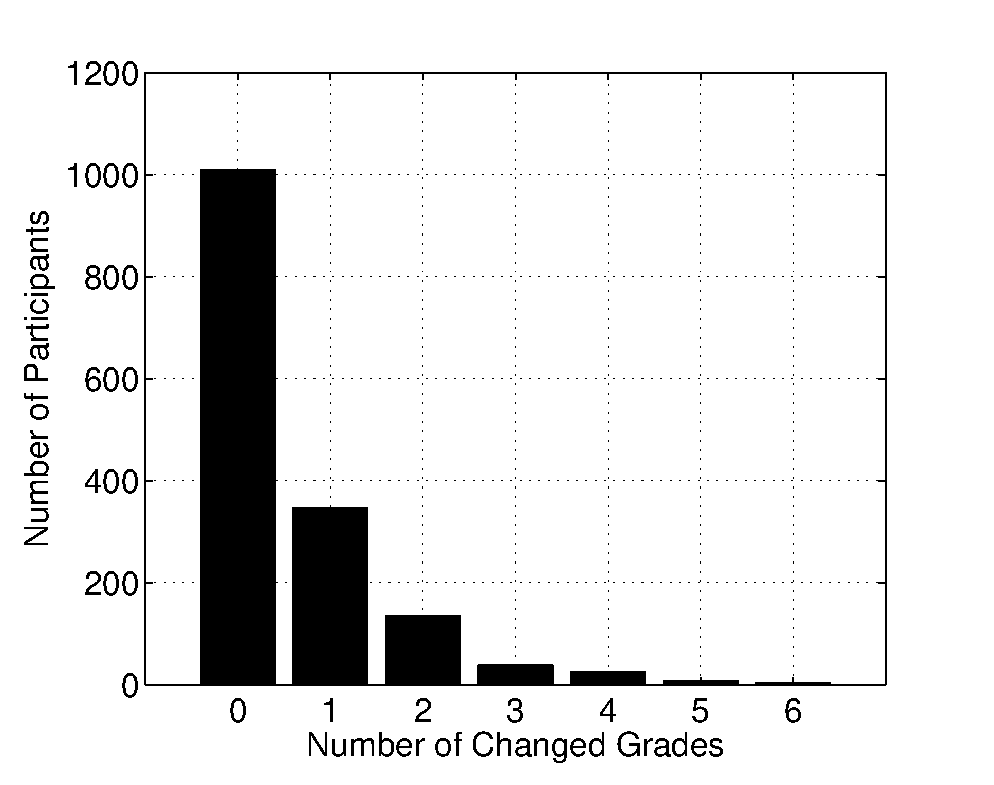
\includegraphics[scale=.25]{../plots/change-1.eps}
    \hspace*{-2em}
    \includegraphics[scale=.25]{../plots/change-2.eps}
      \caption{The majority of participants did not change grades. 65\% change none of their grades, 22.0\% changed one, 8.6\% changed two, and only 6.5\% changed three or more. The lower figure shows that majority of grade changes were towards the median grade rather.}
      \label{change-1}
\end{figure}

\subsection{Moving Towards the Median}
Using the non-parametric test proposed in Section \ref{ht}, we tested the hypothesis of whether grade changes led to significantly more concentration around the median grade.
In our first experiment (Figure \ref{mdev-1}), we tested the absolute deviations of only the CRC participants.
We compared the group of participants that did not change their grades to the group that changed their grades.
We found that while there were no statistically significant differences between the initial grades of the two groups, the final grades of the group that changed were statistically significantly more concentrated than both their own initial grades and the grades of the no change group.
For the set of participants who changed their grades $P_c$ and those who did not $P_n$:
\begin{figure}[h]
\centering
    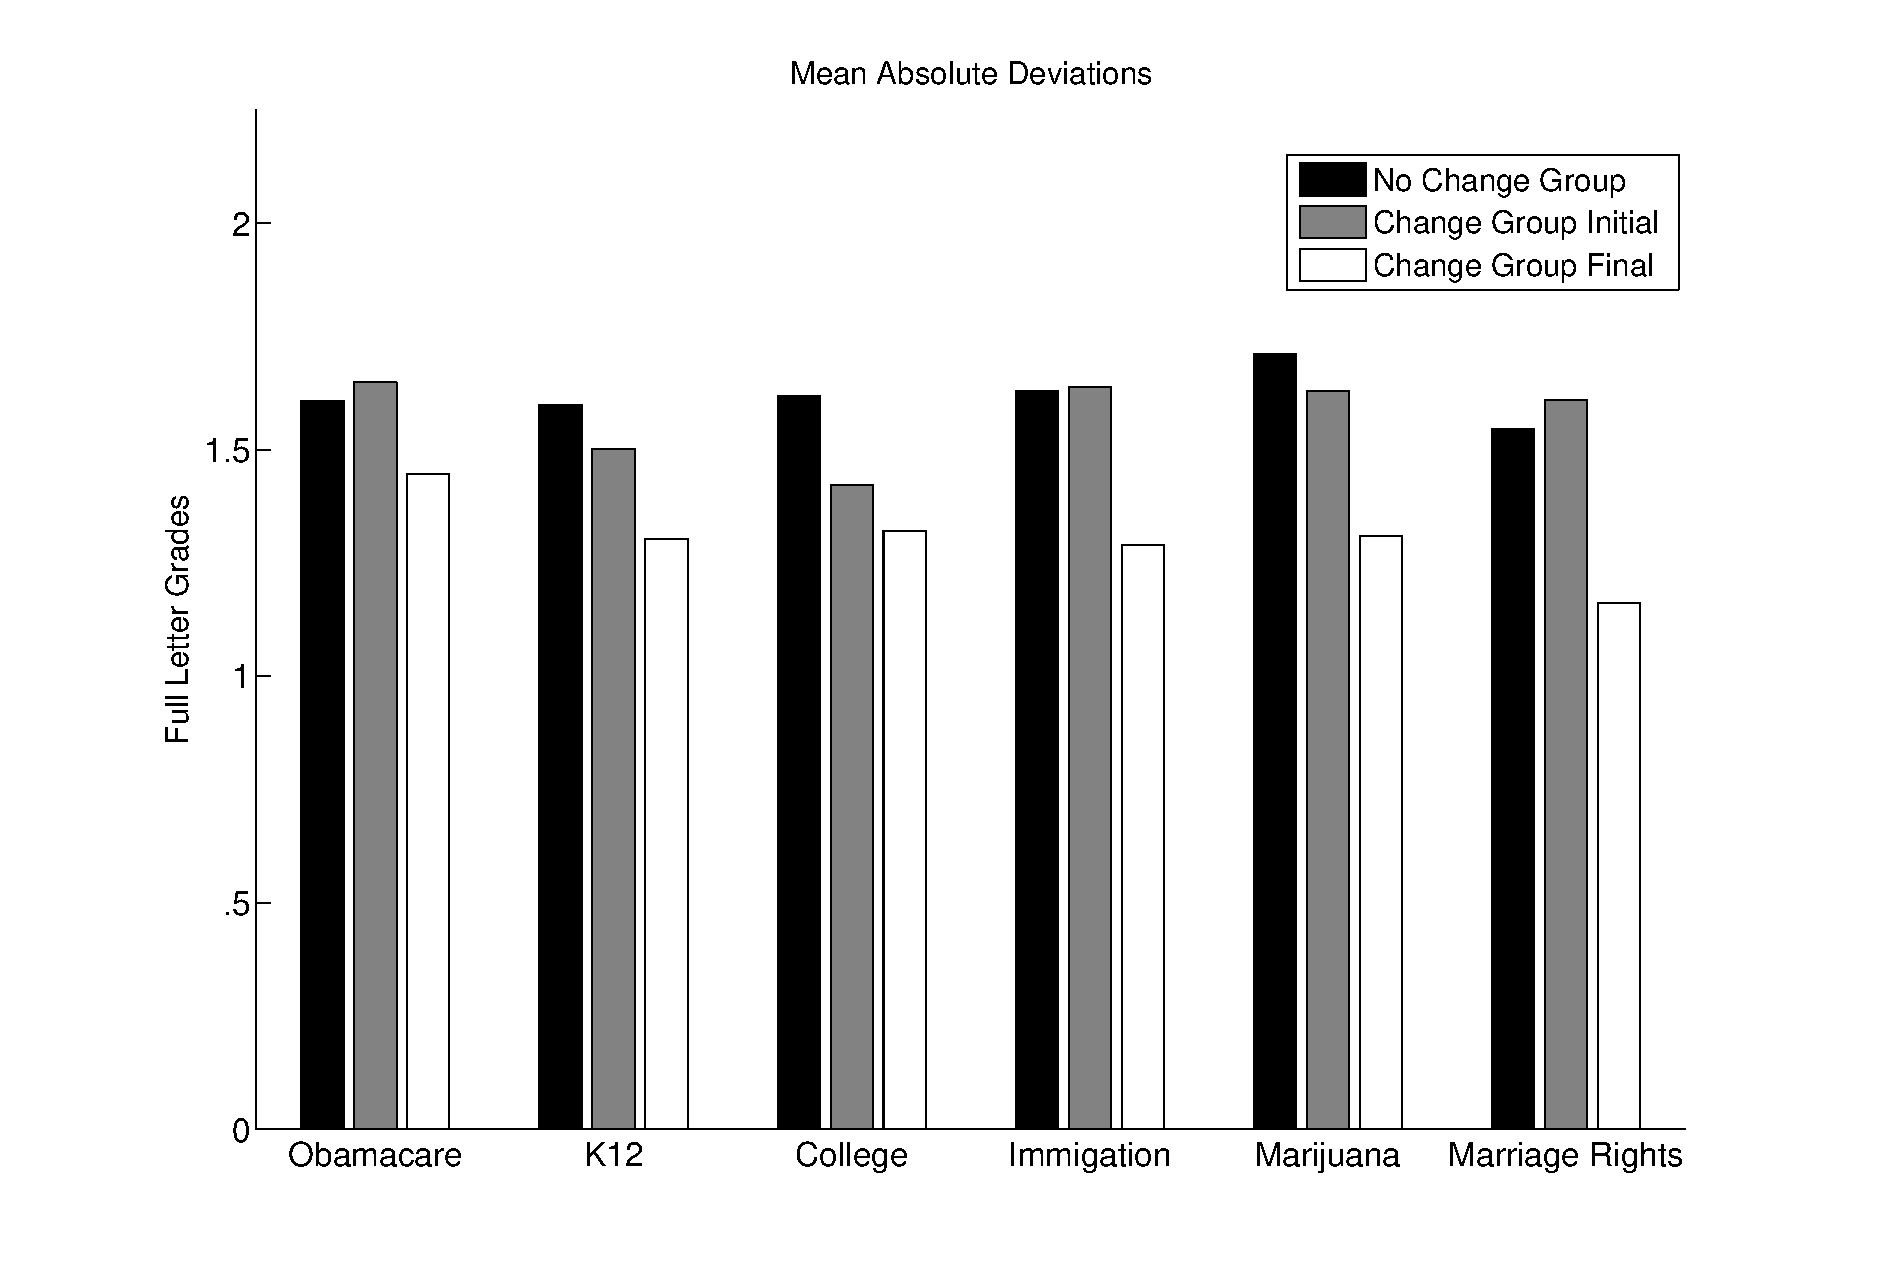
\includegraphics[scale=0.24]{../plots/abs-deviations-1.eps}
      \caption{For those participants that changed their grades, final grades were significantly more concentrated around the median grade than their initial grades. In addition, these grades are more concentrated than the grades for those who didn't change.}
      \label{mdev-1}
\end{figure}

{\centering
\scriptsize
\begin{tabular}[!ht] { r | r | r }
\label{dev-2}
  Issue & p-val($P_c$ vs. $P_n$) & p-val($i$ vs. $f$) \\
  \hline
  \hline
  Obamacare &  0.0286 & 0.0161 \\
  \hline
  K12 & 2.1314e-06 &  0.0086 \\
  \hline
  College & 1.3033e-04 & 0.0415 \\
  \hline
  Immigration & 7.3456e-07 &4.4170e-05\\
  \hline
  Marijuana & 2.7549e-10 & 4.2560e-05\\
  \hline
  Marriage Rights & 3.5946e-06 & 2.4644e-10 \\
\end{tabular}\\[1\baselineskip]
}

These results are consistent with social influence bias.
When participants change their grades, they are more likely to concentrate around the median.
What is particularly surprising is that the two groups of participants $P_n$ and $P_c$ are very similar in terms of initial grades, and the data suggests that a participant's susceptibility to social influence is not correlated with initial grades.

In our second experiment (Figure \ref{mdev-2}), we apply the same testing procedure to compare the grades from the CRC to to those in the reference survey.
We compare absolute deviations of the group of participants who changed their grades in the CRC against participants from the reference survey.
\begin{figure}[h]
\centering
    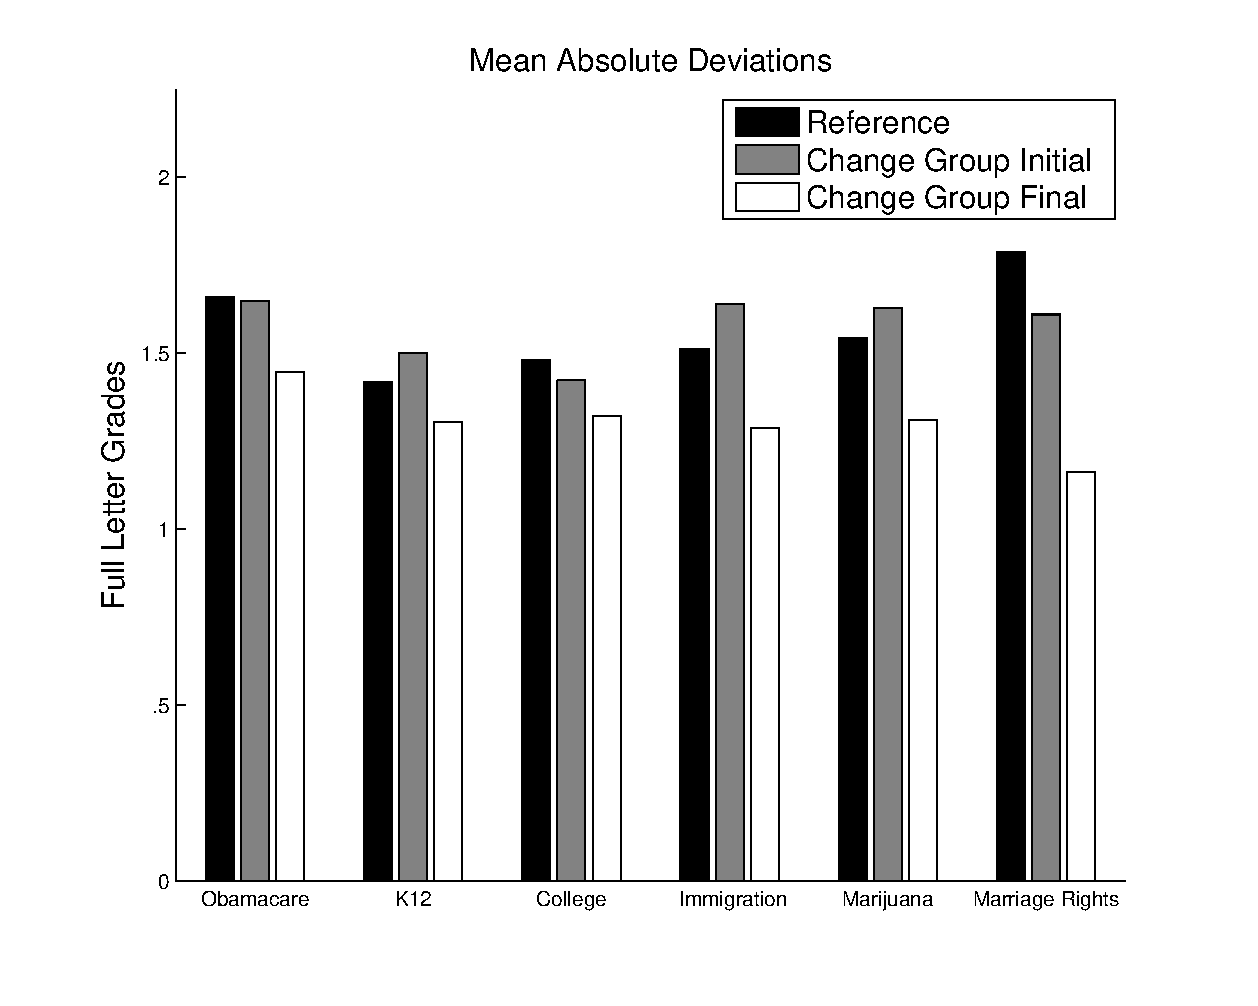
\includegraphics[scale=0.24]{../plots/bias-2.eps}
      \caption{We found that final grades were significantly more concentrated in the CRC compared to grades in the reference survey. Similar to Figure \ref{mdev-1}, we found that there was no statistically significant difference between the reference survey and the initial grades.}
      \label{mdev-2}
\end{figure}

{\centering
\scriptsize
\begin{tabular}[!ht] { r | r | r }
\label{ref-1}
  Issue & p-val($R$ vs. $i$) & p-val($R$ vs. $f$) \\
  \hline
  \hline
  Obamacare &  0.5386 & 0.0015 \\
  \hline
  K12 & 0.8283 & 0.0097 \\
  \hline
  College & 0.1452 & 0.0091 \\
  \hline
  Immigration & 0.3765 & 1.1787e-04\\
  \hline
  Marijuana & 0.7288 & 9.3111e-06\\
  \hline
  Marriage Rights & 0.2478 & 0.0161 \\
\end{tabular}\\[1\baselineskip]
}

The results of our two experiments are consistent with social influence bias.
We not only found that participants' changed grades were statistically significantly more likely to concentrate around the median, they were also more likely in comparison to the reference survey.
While correlation does not imply causation, we argue that this evidence rejects the null hypotheses and is most consistent with \textbf{Hypothesis 1}.
As the CRC was not a randomized survey, there are possibly confounding covariates eg. participants who changed their grades were more likely to leave tightly concentrated grades in the first place.
However, our comparison with the reference survey, and discovery that initial grades were largely consistent with the reference survey and with those that didn't change their grades, suggest that these confounding covariates are not very significant.
These results are encouraging and we hope to run a randomized participant study to confirm a causal relationship.

\subsection{Correlation vs. Absolute Deviation}
\label{exp-robust}
We ran an experiment to illustrate the problems of using correlation instead of absolute deviation.
In this experiment, we iterated through the initial grades each of participants in the change group $P_c$.
For each grade, we randomly sampled a final grade from group $P_n$.
In this model, since we sample final grades from the no change group, we know that the social influence bias hypothesis is not true.
However, when we calculate the correlation coefficient between $g_f[j] - m[j]$ and $g_i[j] - m[j]$, we find statistically significant correlations.

{\centering
\scriptsize
\begin{tabular}[!ht] { r | r | r }
\label{ref-2}
  Issue & corr & p-val \\
  \hline
  \hline
  Obamacare &  0.709 & 5.2e-56 \\
  \hline
  K12 & 0.659 & 4.73e-38 \\
  \hline
  College & 0.673 & 2.26e-36 \\
  \hline
  Immigration & 0.704 & 2.95e-32\\
  \hline
  Marijuana & 0.689 & 1.42e-34\\
  \hline
  Marriage Rights & 0.679 & 3.27e-41 \\
\end{tabular}\\[1\baselineskip]
}
There is a natural tendency for grades to group around the median grade and the correlation coefficient does not account for this.
However, if we measure the absolute deviation, we will find there is no statistically significant difference between the absolute deviations since they are sampled from the same group.
\subsection{Estimating the Social Influence Bias}
\begin{figure}[ht!]
\centering
    \includegraphics[scale=0.22]{../plots/shift-parameter.eps}
      \caption{We calculate the shift-parameter $\Delta$ which is the distance from the null hypothesis. Over all issues, we found that on average grades were more than 1/3 of a letter grade closer to the median.}
      \label{shift-1}
\end{figure}
We tested the hypotheses and conclude significant additional concentration of grades around the median grade.
In Section \ref{ht}, we described how we could use the results of the hypothesis test to estimate the $\Delta$ parameter, which quantifies how different the hypothesis is from the null distribution (no social influence bias).
We use $\Delta$ as a measure of social influence bias.

In Figure \ref{shift-1}, we show the parameter estimates for each of the issues.
As before, the units of the plot are in terms of letter grades.
For the issues about Marriage Rights, we find that parameter is 2/3 of a letter grade.
This means that the set of absolute deviations for the change group $X_c$ was on average 2/3 of a letter grade smaller.
For the other issues, the parameter was smaller indicating less of an effect of social influence bias.
On average over all issues, the grades were $0.3889$ full letter grades closer to the median, which corresponds to 8.9\% on a normalized absolute scale.

\subsection{Sequential Evolution of Social Influence}
Using the model proposed in Section \ref{path}, we calculated the test statistics for both the CRC and the Reference Survey.
Recall, that this model calculates the change in disagreement with the median; that is, how much did a participant disagree with the median on past responses compared 
to the current value.
A comparatively larger value in the CRC suggests repeated feedback of the median grade encourages future responses to be more moderate.
Figure \ref{path-1} illustrates the results of the experiment for the five last issues (K12, College, Immigration, Marijuana, Marriage Rights), and using the mean disagreement on the previous issues.
We see that for the last three issues the change in disgreement is comparatively much higher in the CRC.
The experimental results were not as significant as the other experiments and we found that only two issues Immigration (p=0.0037) and Marijuana (p=0.0287) showed an order dependence that was significantly greater than the reference survey.
In summary, we were not able to reject the null hypothesis for all issues, but we did find some indication that ordering plays an important role, at least for the later issues.

\begin{figure}[h]
	\centering
    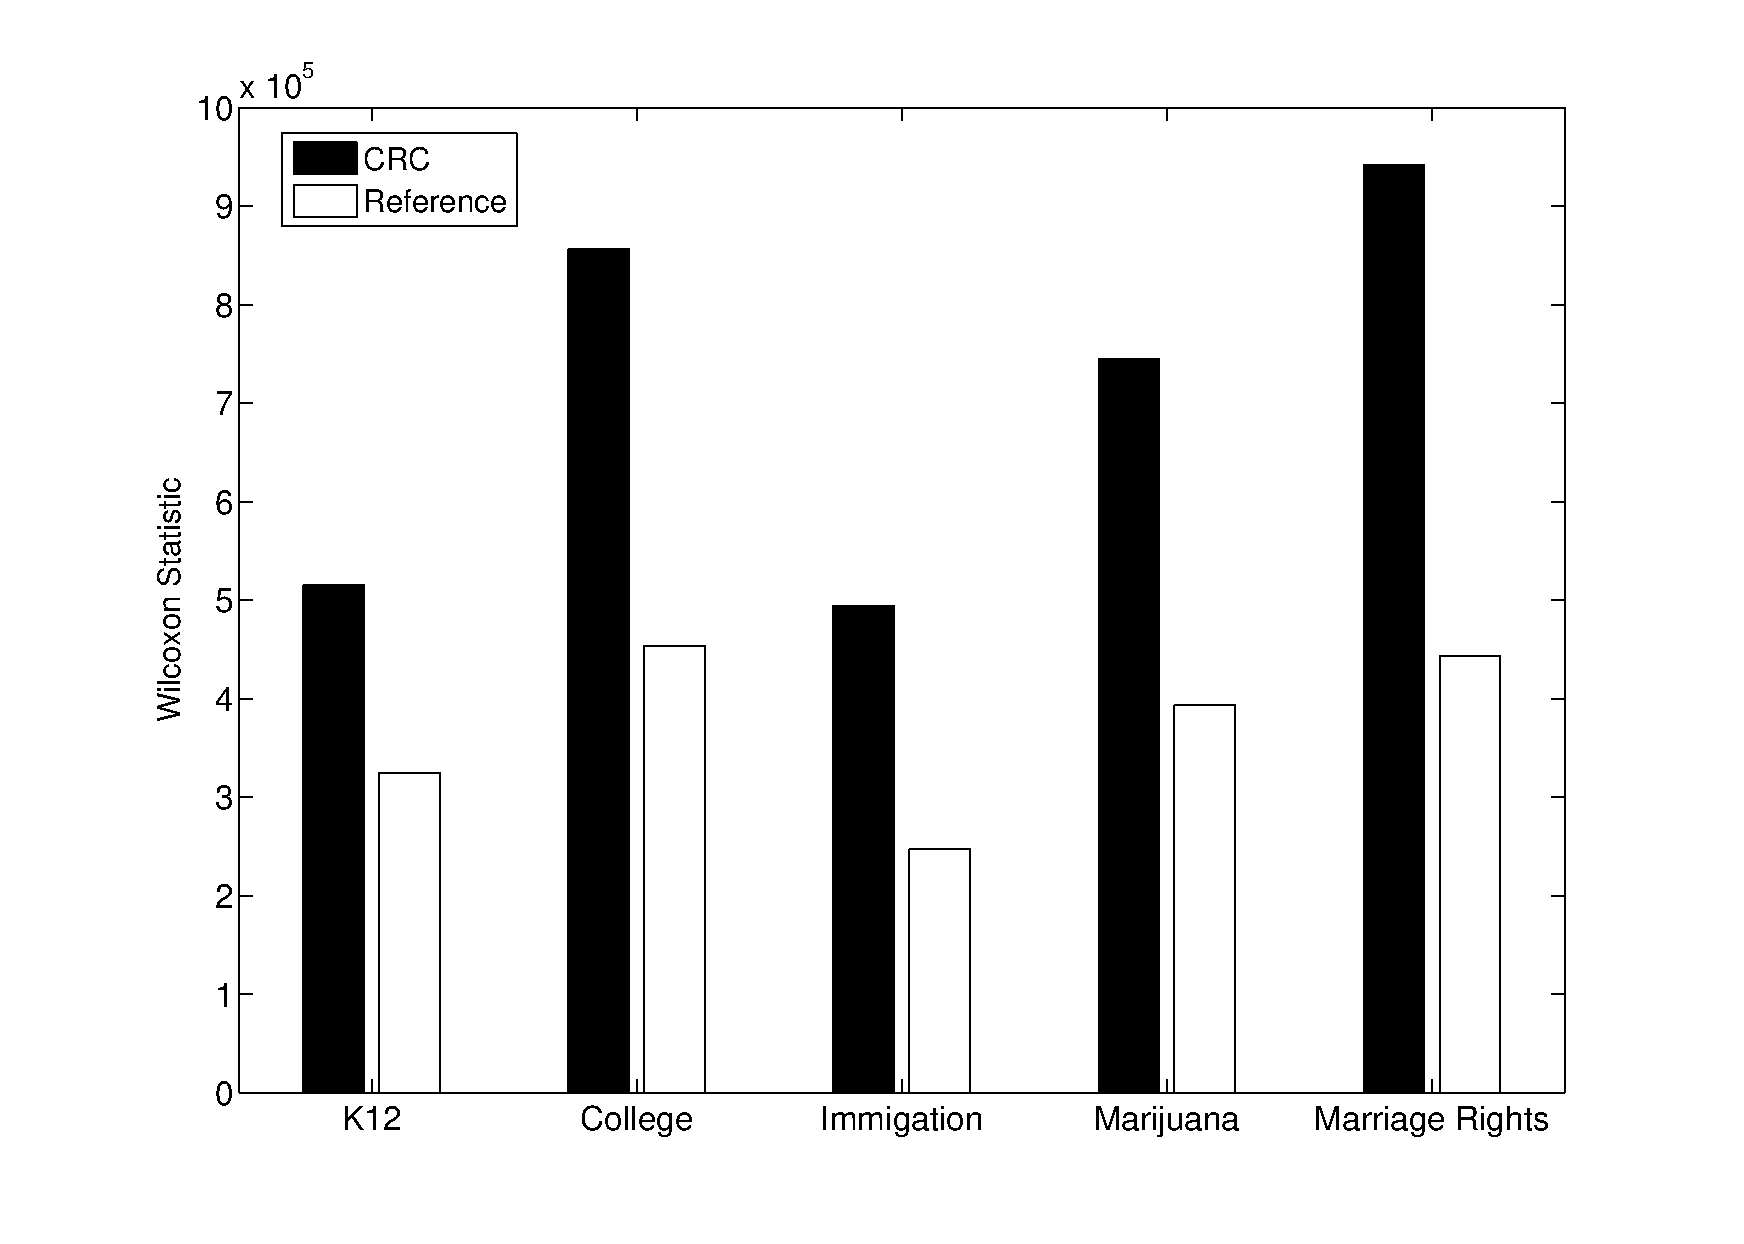
\includegraphics[scale=0.24]{../plots/path-dependence.eps}
      \caption{We measure the mean change in disagreement for each issue. The change in disagreement is defined as the average deviation with median on previous issues minus the deviation with the median on the current issue. We hypothesized that the CRC would have comparatively greater (or less negative) values than the reference survey.}
      \label{path-1}
\end{figure}

\begin{figure*}[ht!]
\hspace{-7em}
    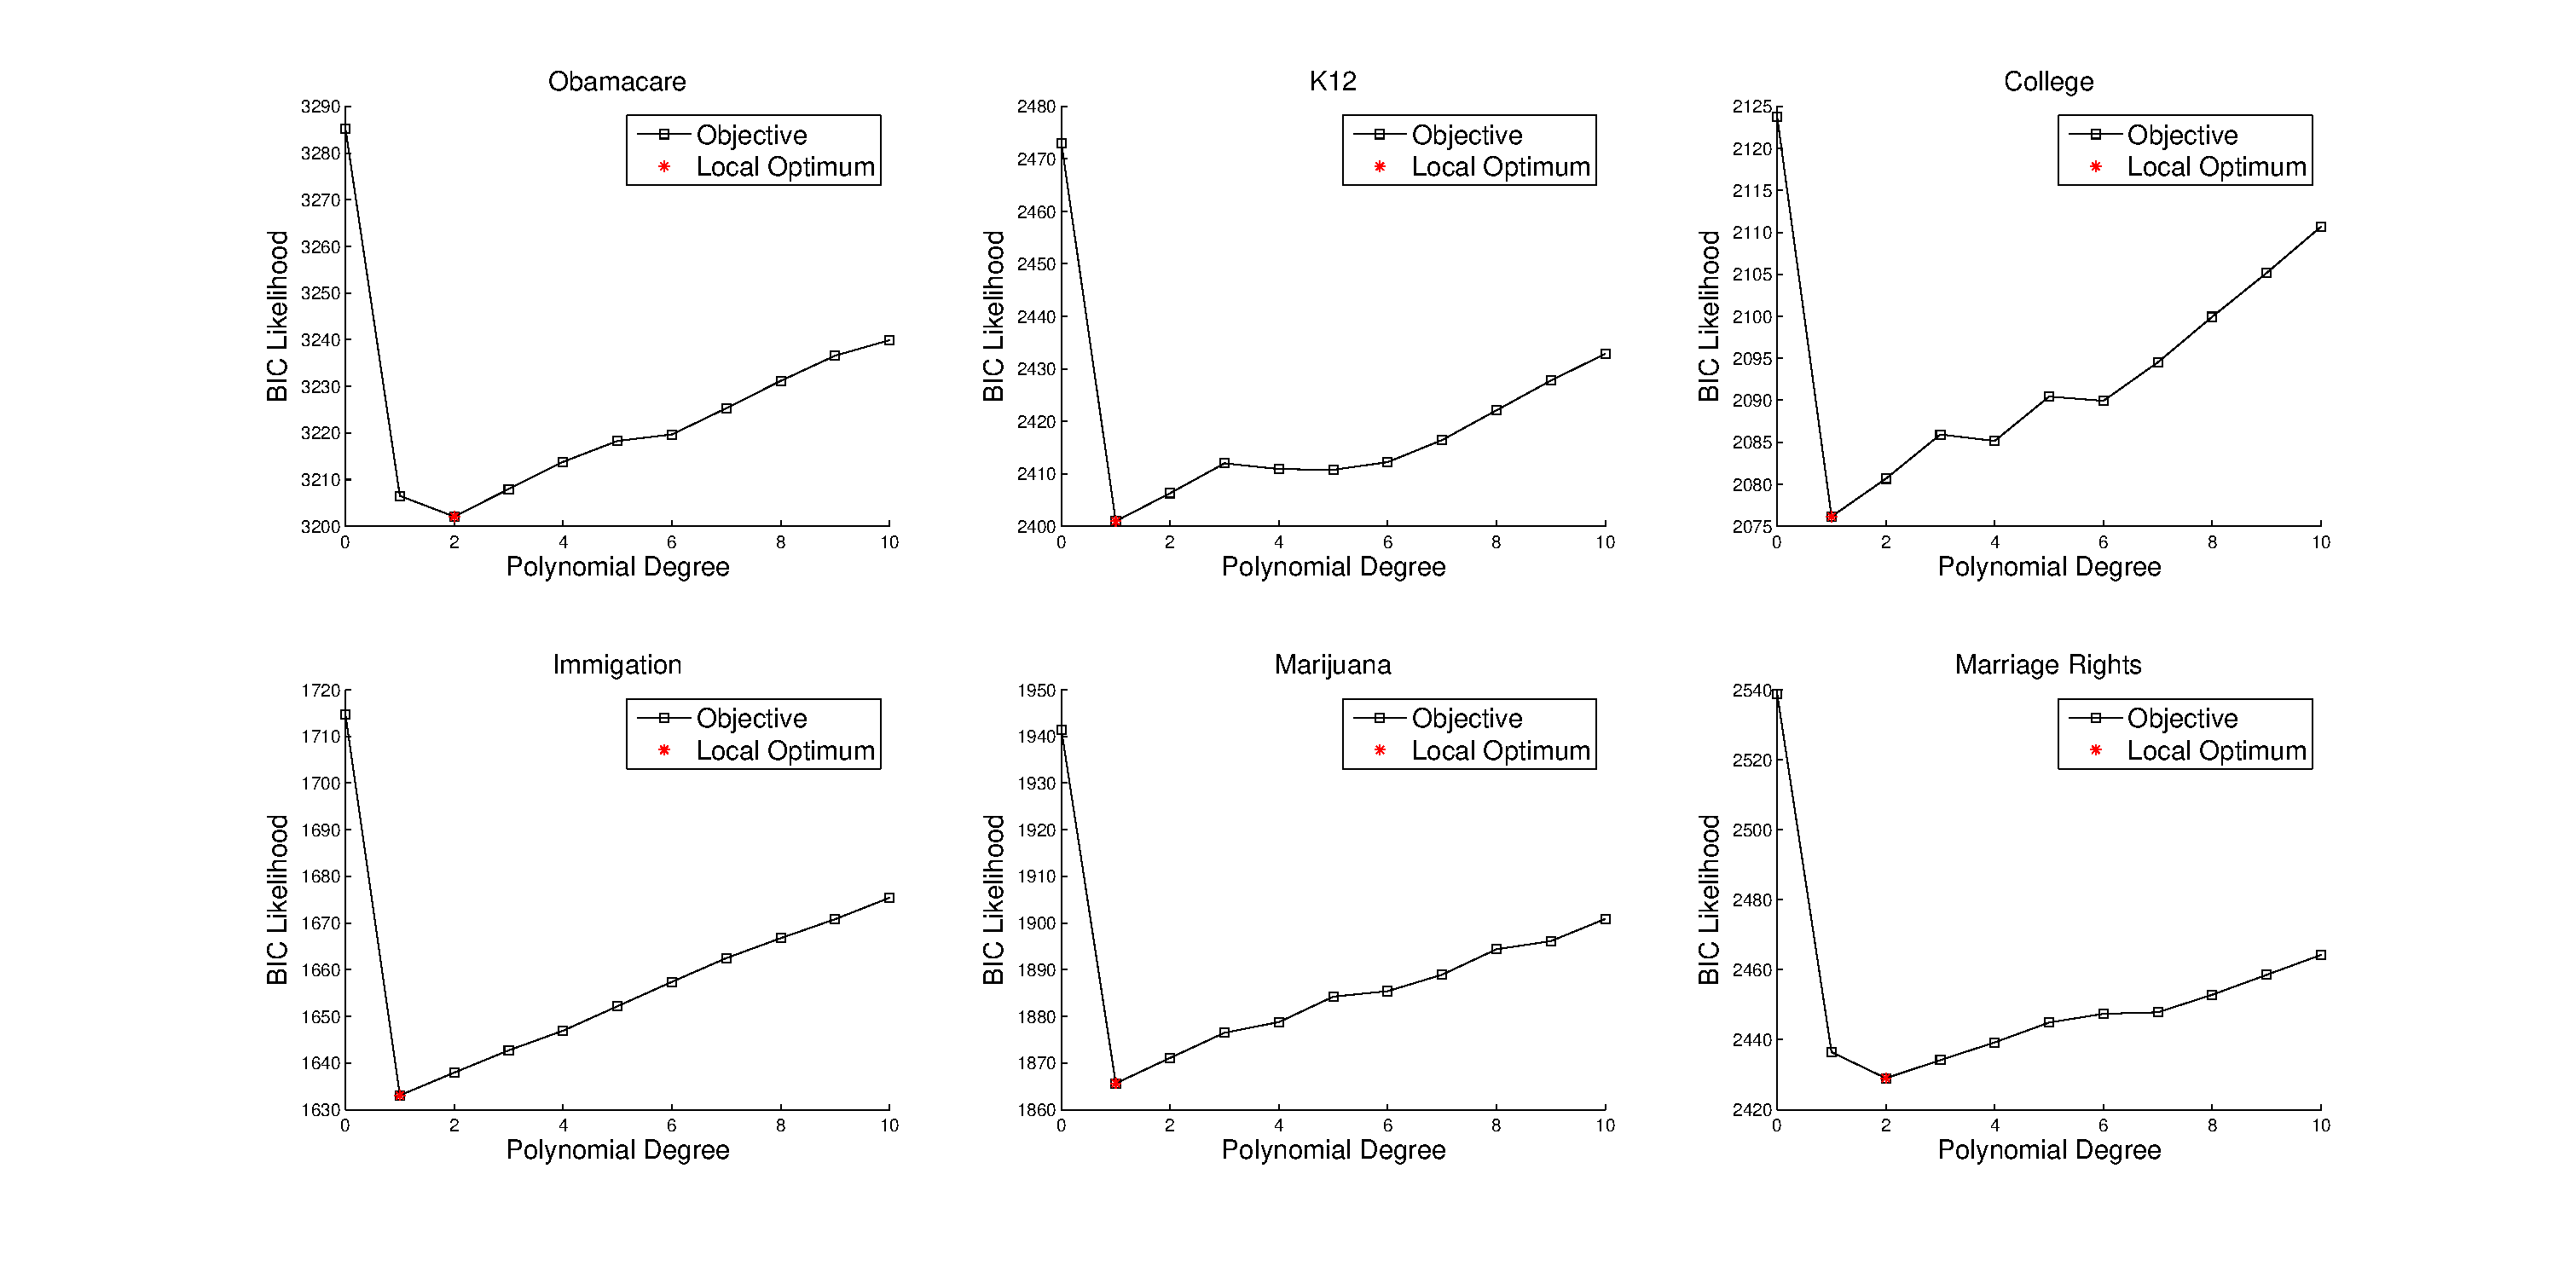
\includegraphics[scale=0.35]{../plots/BIC-optimization.eps}
      \caption{For the participants that changed their grades, we plot the difference between their grade and the median (X-axis), and their changed grade (Y-axis). We overlay the optimal polynomial model to represent the relationship $f(x) = y$. Below each plot, is the BIC objective function showing how we picked an optimal degree of polynomial.}
      \label{opt-1}
\end{figure*}
\subsection{Predicting Grade Changes}
We train the polynomial model proposed in Section \ref{changemod}, and the results are shown in Figure \ref{opt-1}.
Our model search and optimization through the BIC discovered that for four out of the six issues, K12, College, Immigration, and Marijuana, the model was linear.
This suggests homogeneity in positive and negative social influence effects for these issues.
What this implies is that on average participants who graded above the median and below the median moved towards the median with the same magnitude.
However, for Obamacare and Marriage Rights, we found that the relationship was quadratic.
Interestingly enough, over the domain of changes, the learned quadratic function was ``almost" linear, but with a steeper curve for grades above the median.
Participants who initially graded the state higher than the median had a more significant tendency to change downwards, in comparison to the upward tendency of those who graded less than the median.

These models further illustrate the subtlety and context dependence of social influence bias. 
In Muchnik et al. they observed a biasing tendency where both positive and negative influence led to increased upward bias (due to conforming and correcting tendencies respectively).
Compared to those results, our results are quite different as we observe movement towards the median for both positive and negative influences.

We also tested our model in terms of RMSE prediction error (Figure \ref{poly-1}). 
We held out 20\% of the pairs of ratings (observed change, actual) and tested the prediction error on this held out set.
We found that our model on average, over all issues, predicted final grade within $0.5150$ letter grades, or 11.8\% on a normalized absolute scale.
Note that 1/3 of a letter grade corresponds to the difference of just a + or - grade.

In a second experiment (Figure \ref{poly-1}), we applied the inverse model to infer initial grades from the final ones.
We measured the performance of the inverse model by re-caluating the $\Delta$, which can be interpreted as a distance from the null hypothesis of no social influence bias, for the predicted initial grades.
A $\Delta$ of 0 means that the null hypothesis of no social influence bias cannot be rejected, thus indicating perfect correction.
We found that there was on average a 76.3\% reduction in $\Delta$ which quantifies the concentration around the median. 
While the bias is still statistically significant, it is greatly reduced and the spread of participants around the median grade better reflects the initial grades.

\begin{figure}[h]
\hspace*{-2em}
    \includegraphics[scale=0.25]{../plots/prediction-error.eps}
    \hspace*{-2em}
    \includegraphics[scale=0.24]{../plots/shit-2.eps}
      \caption{We measured the RMSE prediction error of the polynomial model. We found that we could predict changes in all of the issues with less than 2/3 of a letter grade RMSE error. In the lower figure, we applied this model to correct for the social influence bias and found that, on average, we could reduce the effects by 76.3\%}
      \label{poly-1}
\end{figure}





\section{Future Work}
The methods we proposed have several interesting directions of future interest. 
We want to extend our work to quantify biases in textual data. 
The California Report Card collects textual suggestions from participants in addition to the quantiative assesment results. 
Participants are encouraged to read the responses of others before leaving a suggestion of their own.
We suspect that this may lead to a bias in the topics discussed by participants, and we would like to explore how similar non-parametric models can be extended to textual data.

Another compelling direction is to attempt to parameterize our model.
We will explore whether we can model the grades as a mixture of binomial distributions (a discrete analog of a mixture of gaussians), and try to derive optimal tests and models for this data.
Intuitively, parametrization should lead to increased statistical power and better fitting models; assuming that the data fits the underlying parametrization.

\section{Conclusion}
We proposed non-parametric hypothesis tests and models to evaluate the biasing tendency of visible aggregate statistics in the California Report Card.
We found that revealing the median led to a statistically significantly tighter grouping of grades around the shown median grade.

We modeled the biasing effect as a regression towards the median grade and fit polynomial to represent the functional relationship between a participant's observed difference with the median and then subsequent grade change.
We applied an information theoretic criteria to select a model of appropriate complexity.
We found that this relationship was quadratic in two out of the six issues, representing a heterogeneity in biasing for positive and negative differences with the median.
We further showed how non-parametric ideas could be extended to the problem of Wilcoxon shift parameter estimation and quantify the effects of the biasing tendency.

In principle, the methods we proposed can be applied to test and model biases in a wide variety input mechanisms.
This is a key motivation for our non-parametric approach.
Understanding these biases, can give insight into the behavior of recommender systems that train on such data.

%\end{document}  % This is where a 'short' article might terminate


%
% The following two commands are all you need in the
% initial runs of your .tex file to
% produce the bibliography for the citations in your paper.
{
\bibliographystyle{abbrv}
\fontsize{7.1pt}{7.0pt} \selectfont
\bibliography{sigproc}  % sigproc.bib is the name of the Bibliography in this case
}
% You must have a proper ".bib" file
%  and remember to run:
% latex bibtex latex latex
% to resolve all references
%
% ACM needs 'a single self-contained file'!
%
%APPENDICES are optional
%\balancecolumns

\balancecolumns
% That's all folks!
\end{document}
